\documentclass[tikz]{standalone}
\usepackage{pgfplots}
\pgfplotsset{compat=1.15}
\usepackage{mathrsfs}
\usetikzlibrary{arrows,calc}
\usepackage{tkz-euclide}

\pagestyle{empty}

\definecolor{AngleClr}{rgb}{0,0.39215686274509803,0}
\definecolor{ShapeClr}{rgb}{0.6,0.2,0}

\begin{document}

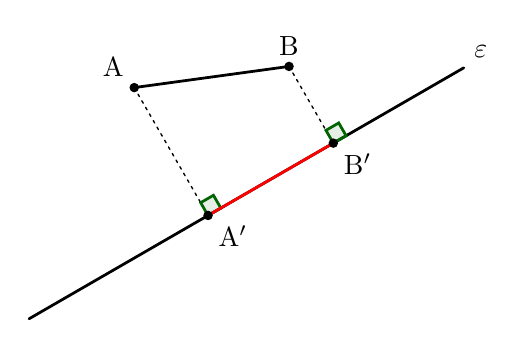
\begin{tikzpicture}[scale=.75]
\tkzSetUpLine[line width=1pt,color=black]
\tkzSetUpPoint[fill=black]

\tkzDefPoints{0/0/O}

\tkzDefPoint(30:5){x'}
\tkzDefPoint(-150:3.5){x}
\tkzDefPoint(-60:1.75){y}
\tkzDefPoint(120:2.5){y'}

\tkzDefPointOnLine[pos=-0.4](x,x')\tkzGetPoint{eps}

\tkzDefPointOnLine[pos=0.7](x,x')\tkzGetPoint{OO}

\begin{scope}[shift=(OO)]
\tkzDefPoint(30:6){xx'}
\tkzDefPoint(-150:3.5){xx}
\tkzDefPoint(-60:1.75){yy}
\tkzDefPoint(120:1.5){yy'}

\end{scope}

\tkzDrawSegments[line width=1pt,color=black](x,x' y',yy')

\tkzDrawSegments[line width=0.5pt,color=black,dashed,dash pattern=on 1pt off 1.75pt](y',O yy',OO)

\tkzMarkRightAngles[line width=1pt, size=.25,color=AngleClr,fill=AngleClr,fill opacity=0.1](y',O,x' yy',OO,xx')
\tkzDrawSegments[line width=1pt,color=red](O,OO)

\tkzDrawPoints[size=3](y',O,yy',OO)
\tkzLabelPoint[below right](O){$\rm A'$}
\tkzLabelPoint[above right](x'){$\varepsilon$}
\tkzLabelPoint[above left](y'){$\rm A$}
\tkzLabelPoint[below right](OO){$\rm B'$}
\tkzLabelPoint[above](yy'){$\rm B$}

\end{tikzpicture}

\end{document}
